\documentclass{article}
\usepackage{listings}
\usepackage{graphicx}
\usepackage{adjustbox}
\usepackage{amsmath}

\begin{document}
\begin{enumerate}
\item \begin{minipage}[t]{\linewidth}
          \raggedright
          \adjustbox{valign=t}{%
            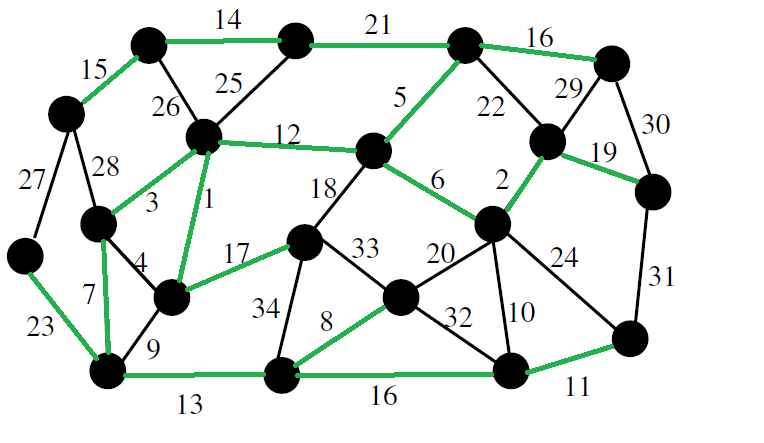
\includegraphics[width=.8\linewidth]{one.png}%
         	 }
	\end{minipage}
\item \begin{minipage}[t]{\linewidth}
          \raggedright
          \adjustbox{valign=t}{%
            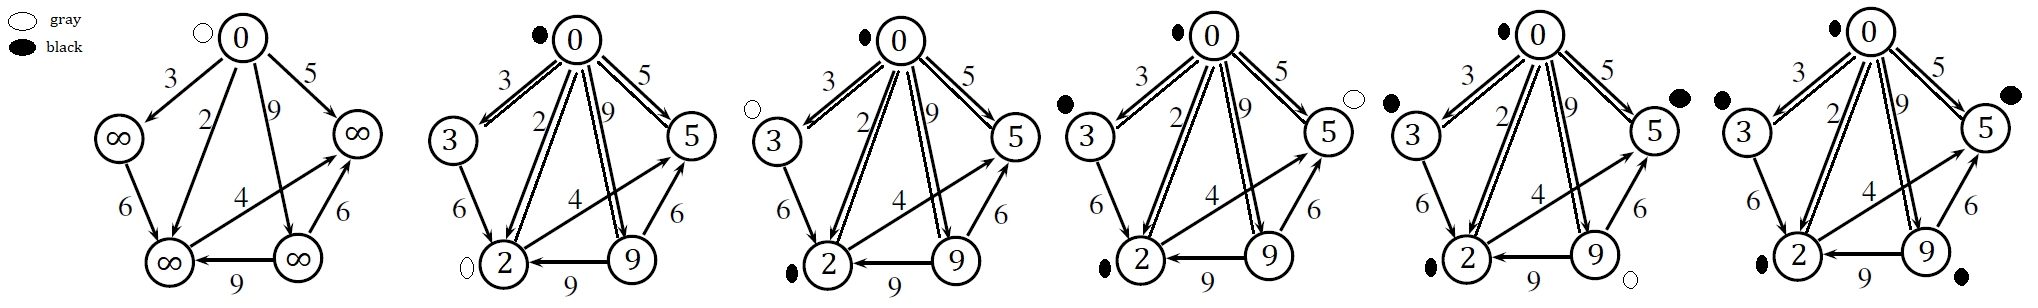
\includegraphics[width=.8\linewidth]{two.png}%
         	 }
	\end{minipage}
\item \begin{lstlisting}
int[][] tc = all 0s
void transitiveClosure()
{
    for (int i = 0; i < V; i++)
        DFS(i, i); //modified depth-first search
 
    for (int i = 0; i < V; i++)
    {
        for (int j = 0; j < V; j++)
            print(tc[i][j] + " ");
        println();
    }
}
void DFS(int a, int b)
{
    tc[a][b] = 1;
 
    // find all vertices reachable through b
    for each int i in adj[b] {
        if (tc[a][i] == 0)
            DFS(a, i);
    }
}
	\end{lstlisting}
\item I'm assuming 0-based indexing:
	\begin{equation*}D^{(1)}=\begin{pmatrix}
	0 & 5 & \infty & 3\\\infty & 0 & -1 & \infty\\ 6 & \infty & 0 & \infty\\2 & 2 & 1 & 0
	\end{pmatrix}\end{equation*}
	\begin{equation*}D^{(2)}=\begin{pmatrix}
	0 & 5 & \infty & 3\\5 & 0 & -1 & \infty\\6 & \infty & 0 & \infty\\2 & 2 & 1 & 0
	\end{pmatrix}\end{equation*}
	\begin{equation*}D^{(3)}=\begin{pmatrix}
	0 & 5 & 4 & 3\\5 & 0 & -1 & \infty\\6 & \infty & 0 & \infty\\2 & 2 & 1 & 0
	\end{pmatrix}\end{equation*}
	\begin{equation*}D^{(4)}=D^{(3)}\end{equation*}
\end{enumerate}
\end{document}
